% SPDX-FileCopyrightText: 2026 Clyde Laforge <clyde.laforge@cern.ch>
% SPDX-License-Identifier: CC-BY-4.0

\documentclass{cernatsnote}

\setlength{\marginparwidth}{2cm}
\usepackage[colorinlistoftodos]{todonotes}
\usepackage{placeins}
\usepackage{multicol}
\usepackage{siunitx}
\usepackage{abstract}
\usepackage{tikz}
\usepackage{booktabs}
\usepackage{multirow}
\usepackage{hyperref}
\usepackage{subcaption}

\usepackage{longtable}
\usepackage{circuitikz}

\title{TRIDENT-GF180-TESTSTRUCTURES Datasheet}
\date{\today}
%\setcounter{secnumdepth}{0}

\begin{document}

\renewcommand{\abstractname}{\vspace{-\baselineskip}} % Remove abstract header
\setlength{\absleftindent}{0mm}
\setlength{\absrightindent}{0mm}
\maketitle

\begin{abstract}
\begin{multicols}{2}
\section{Known issues}
\begin{enumerate}
    \item The markings of pin 100, pin 1 and pin 2 are incorrect. Pin 100 marking is actually pin 99. Pin 1 marking is pin 100. Pin 2 marking is pin 1.
\end{enumerate}


\section{Applications}
\begin{itemize}
  \item Leakage evaluation of GlobalFoundries GF180MCU (\texttt{gf180mcuD}) \SI{180}{\nano\meter} process
  \item Evaluation of guard-trace effectiveness
  \item Evaluation of foundry vs. custom guarded ESD pad approaches for ultra-low current measurement
  \item Characterization of discrete HV/LV NFET and PFET leakage under guarding
  \item Characterization of MIM capacitor leakage and perimeter effects
  \item Evaluation of picoampere two-transistor charge-pump / current generator structure
\end{itemize}

\section{Description}
TRIDENT-GF180-TESTSTRUCTURES is a dedicated test ASIC to assess feasibility of ultra-low current (pA and below) measurements in \texttt{gf180mcuD}.
It is available open source \href{https://github.com/Scafir/gf180mcu-project-trident-gf180-teststructure}{here}.
The primary metric is control and predictability of leakage current from ``hot'' measurement nodes. Primary leakage paths of interest are ESD protection networks, transistor, MIM capacitor, and leakage through insulator mitigated by driven guards.

Pins between structures are often interleaved, to allow for the neighboring pins to be driven as guard.
This is especially useful when large voltage between pins are expected on the same device, such as the MIM capacitors.


\end{multicols}
\end{abstract}

\section{Block Diagram}
\begin{figure}[h]
    \centering
    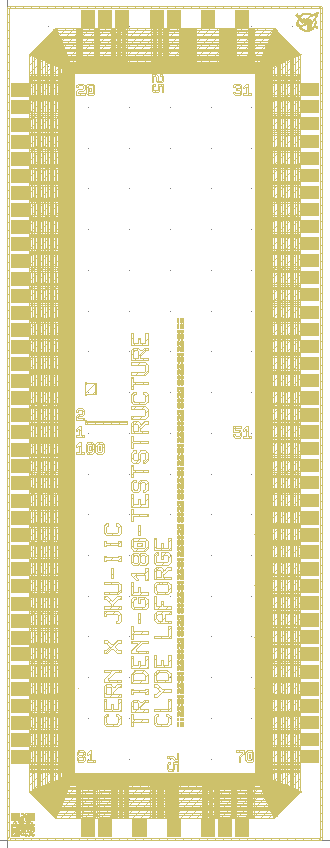
\includegraphics[height=\linewidth, angle=270]{figures/chip_view.png}
    \caption{Top level view of the chip}
    \label{fig:toplevel}
\end{figure}

\pagebreak
\pagestyle{fancy}

\section{Pin Configuration and Function Descriptions}

\begin{longtable}{r l l l}
\toprule
\textbf{\#} & \textbf{Pin name} & \textbf{Decription} & \\
\midrule
1  & MC\_MAX\_P1     & MIM capacitor, max perimeter, terminal P1\\
2  & MC\_MIN\_P2     & MIM capacitor, min perimeter, terminal P2\\
3  & MC\_MIN\_P1     & MIM capacitor, min perimeter, terminal P1\\
4--7 & UNUSED        & Do not connect\\
8  & MC\_GUARD\_P2   & Guard for MIM capacitor terminal P2\\
9--13 & UNUSED       & Do not connect\\
14 & GL\_TOP         & Guard leakage structure, top guard\\
15 & GL\_BOT         & Guard leakage structure, bottom guard\\
16 & GL\_SIDE        & Guard leakage structure, side guard\\
17 & GL\_HOT         & Guard leakage structure, hot node\\
18 & GL\_PAD\_GUARD  & Guard leakage structure, guard of hot bondpad\\
19 & VSS             & Ground supply\\
20 & VDD             & Positive supply\\
21 & PESD\_GS\_HOTN    & Pad ESD (guard+sense), inverted hot output\\
22 & PESD\_GS\_SENSEN  & Pad ESD (guard+sense), inverted sense output\\
23 & PESD\_GS\_SENSE   & Pad ESD (guard+sense), sense input\\
24 & NO\_BOND        & No bondpad present, do not bond\\
25 & PESD\_GS\_HOT    & Pad ESD (guard+sense), hot input\\
26 & NO\_BOND        & No bondpad present, do not bond\\
27 & PESD\_G\_HOTN    & Pad ESD (guard), inverted hot output\\
28 & NO\_BOND        & No bondpad present, do not bond\\
29 & PESD\_G\_HOT     & Pad ESD (guard), hot input\\
30 & PESD\_GUARD     & Guard for all PESD structures\\
31 & VSS             & Ground supply\\
32 & VDD             & Positive supply\\
33--48 & UNUSED       & Do not connect\\
49 & DESD\_VDD\_K     & Discrete ESD diodes to VDD, cathode\\
50 & DESD\_VSS\_K     & Discrete ESD diodes to VSS, cathode\\
51 & DESD\_VDD\_A     & Discrete ESD diodes to VDD, anode\\
52 & DESD\_GUARD     & Guard for discrete ESD diode structures\\
53 & VSS             & Ground supply\\
54 & VDD             & Positive supply\\
55 & TR\_GUARD       & Transistor structures, guard (common)\\
56 & TR\_HP\_D       & High-voltage PFET, drain\\
57 & TR\_HP\_G       & High-voltage PFET, gate\\
58 & TR\_HP\_S       & High-voltage PFET, source\\
59 & TR\_HN\_D       & High-voltage NFET, drain\\
60 & TR\_HN\_G       & High-voltage NFET, gate\\
61 & TR\_HN\_S       & High-voltage NFET, source\\
62 & TR\_LP\_D       & Low-voltage PFET, drain\\
63 & TR\_LP\_G       & Low-voltage PFET, gate\\
64 & TR\_LP\_S       & Low-voltage PFET, source\\
65 & TR\_LN\_D       & Low-voltage NFET, drain\\
66 & TR\_LN\_G       & Low-voltage NFET, gate\\
67 & TR\_LN\_S       & Low-voltage NFET, source\\
68 & TR\_GUARD       & Transistor structures, guard (common)\\
69 & VSS             & Ground supply\\
70 & VDD             & Positive supply\\
71 & PL\_GUARD       & Pad leakage structure, guard (common)\\
72 & PL\_FLOAT       & Pad leakage structure, floating pad\\
73 & PL\_GS\_SENSE   & Pad leakage (guard+sense), sense input\\
74 & NO\_BOND        & No bondpad present, do not bond\\
75 & PL\_GS\_HOT     & Pad leakage (guard+sense), hot input\\
76 & NO\_BOND        & No bondpad present, do not bond\\
77 & PL\_G\_HOT      & Pad leakage (guard), hot input\\
78 & NO\_BOND        & No bondpad present, do not bond\\
79 & PL\_A\_HOT      & Pad leakage (analog), hot input\\
80 & PL\_GUARD       & Pad leakage structure, guard (common)\\
81 & VSS             & Ground supply\\
82 & VDD             & Positive supply\\
83 & CP\_GUARD       & Charge pump structure, guard\\
84 & CP\_G2          & Charge pump, gate 2\\
85 & CP\_VS          & Charge pump, VS node (drain+source)\\
86 & CP\_G1          & Charge pump, gate 1\\
87 & CP\_VW          & Charge pump, VW node (bulk)\\
88--96 & UNUSED       & Do not connect\\
97 & VSS             & Ground supply\\
98 & VDD             & Positive supply\\
99 & MC\_GUARD\_P1   & Guard for MIM capacitor terminal P1\\
100& MC\_MAX\_P2     & MIM capacitor, max perimeter, terminal P2\\
\bottomrule
\end{longtable}UNUSED pads are foundry-provided analog ESD pad with their output left unconnected.

NO\_BOND pads have not actual bondpad implemented. They are missing due to the underlying structures being too large.
Instead of simply removing them from lists, they are kept nonetheless  so that the pad positions and numbering stays regular.

\pagebreak
\section{ESD protection pads}

\subsection{Foundry provided analog pad}\label{foundrypad}

Below is a diagram of the foundry provided analog input pad, which provide a classic protection structure.
The input diodes (on the pad side) are very large as they are supposed to take the brunt of the ESD pulses.
The series resistor and output diodes are optional: they are not provided within the pad itself, but users are encouraged to add them in the documentation.
The value of the series resistor is typically a few hundred ohms.
This allow a secondary path for the current in case of an ESD spike, and the series resistor allows for a reduction of the voltage to which the core will be exposed.

This pad has an implementation with no output, to characterize its leakage in ADDREF.
It does not have an implementation with output connected to an inverted to determine its capability of protecting the core transistors due to a lack of time during the layout process.

\begin{circuitikz}
% Supply rails
\draw (0,4) node[vcc]{VDD} -- (8,4);
\draw (0,0) node[ground]{VSS} -- (8,0);

% PAD node and label
\draw (1,2) node[circ,label=left:{PAD}] (pad) {};
\draw (pad) -- (2,2);

% Input clamp diodes (PAD to VDD and VSS)
% To VDD: anode at PAD, cathode at VDD
\draw (2,2) to[diode] (2,4);
% To VSS: anode at VSS, cathode at PAD
\draw (2,0) to[diode] (2,2);

% Series resistor to core/internal node
\draw (2,2) to[R,l=$R_{\mathrm{series}}$] (5,2) -- (6,2) node[circ,label=right:{CORE/IN}] (core) {};

% Output clamp diodes (CORE to VDD and VSS)
% To VDD: anode at CORE, cathode at VDD
\draw (5,2) to[diode] (5,4);
% To VSS: anode at VSS, cathode at CORE
\draw (5,0) to[diode] (5,2);

% (optional) show rails continuing to the right
\draw (5,4) -- (8,4);
\draw (5,0) -- (8,0);

\end{circuitikz}

\subsection{Custom guard pad}\label{guard_pad}

This adds a guard trace around the input trace. This allows for the internal diodes (between PAD and GUARD) to experience a near zero voltage drop, and hence have minimal leakage.
The guard voltage could be driven by a buffer connected to the core voltage.
It could also be driven independently from the input (if it is at a fixed voltage), and trimmed by-device for a specific operating point, likely temperature.

In order to provide somewhat comparable ESD protection to the foundry provided analog pad, the size of each diode is doubled compared to it.

As the inner VSS diode is not connected directly to VSS, it is necessary to put it in a deep N-well.

\begin{circuitikz}
% Supply rails
\draw (0,4) node[vcc]{VDD} -- (9,4);
\draw (0,0) node[ground]{VSS} -- (9,0);

% PAD and CORE nodes
\draw (2,2) node[circ,label=left:{PAD}] (pad) {} -- (3,2);

\draw (3,2) to[R,l=$R_{\mathrm{series}}$] (6,2) -- (7,2)
      node[circ,label=right:{CORE/IN}] (core) {};

% ---- Input diode stacks (two diodes in series each) ----
% PAD -> VDD stack (anodes at PAD, cathodes at VDD)
\draw (3,2) to[diode] (3,3)
      node[circ] (mid_in_vdd) {}
      to[diode] (3,4);

% VSS -> PAD stack (anodes at VSS, cathodes at PAD)
\draw (3,0) to[diode] (3,1)
      node[circ] (mid_in_vss) {}
      to[diode] (3,2);

% ---- Output diode stacks (two diodes in series each) ----
% CORE -> VDD stack
\draw (6,2) to[diode] (6,3)
      node[circ] (mid_out_vdd) {}
      to[diode] (6,4);

% VSS -> CORE stack
\draw (6,0) to[diode] (6,1)
      node[circ] (mid_out_vss) {}
      to[diode] (6,2);

% ---- Guard interconnects ----
% Tie midpoints of VDD stacks together; tie midpoints of VSS stacks together
\draw (mid_in_vss) -- (1,1) -- (0,1) -- (0,3) -- (3,3);

% Connect input-side midpoint (VDD<->PAD) to output-side midpoint (VDD<->CORE)
% through a series resistor (guard resistor)
\draw (mid_in_vdd) to[R,l=$R_{\mathrm{guard}}$] (mid_out_vdd);

\draw (mid_out_vdd) -- (10,3) -- (10,1) -- (6,1);
\draw (10,3) -- (11,3) node[circ,label=right:{GUARD}] () {};

% (optional) rails continuing
\draw (5,4) -- (11,4);
\draw (5,0) -- (11,0);

\end{circuitikz}

\begin{figure}
    \centering
    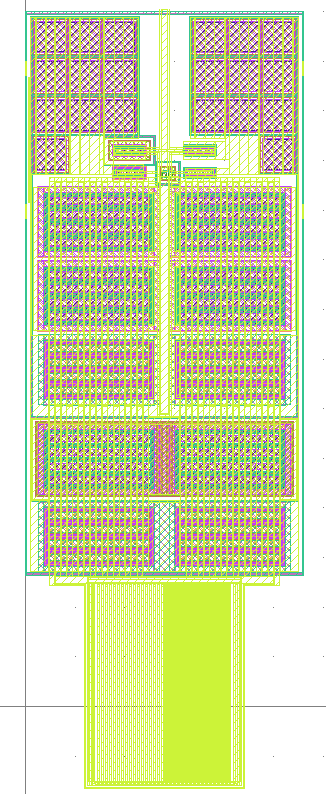
\includegraphics[height=\linewidth,angle=270]{figures/pad_guard_layout.png}
    \caption{A graphic representation of the layout of the custom guard pad}
    \label{fig:custom_guard_pad_layout}
\end{figure}


\subsection{Custom guardsense pad}\label{guardsense_pad}

The custom guardsense pad goes one step further than the custom guarded pad.
It duplicates the internal components (zero-voltage drop diodes and series resistor), and hence provide 2 new ports, named "SENSE" and "CORE SENSE".
Because the implementation of the sense and pad is fully symmetric and interleaved, any leakage experience on the PAD line should be the same on the sense line, provided minimal voltage drop on the series resistor.

This allows for sensing the leakage of the pad input from the core sense.
In turn, a the guard voltage can be dynamically adjusted for zero leakage.

For the layout, it was necessary to implement custom ESD diodes, so that it was possible to interleave the guard and hot signals.

\begin{figure}
    \centering
    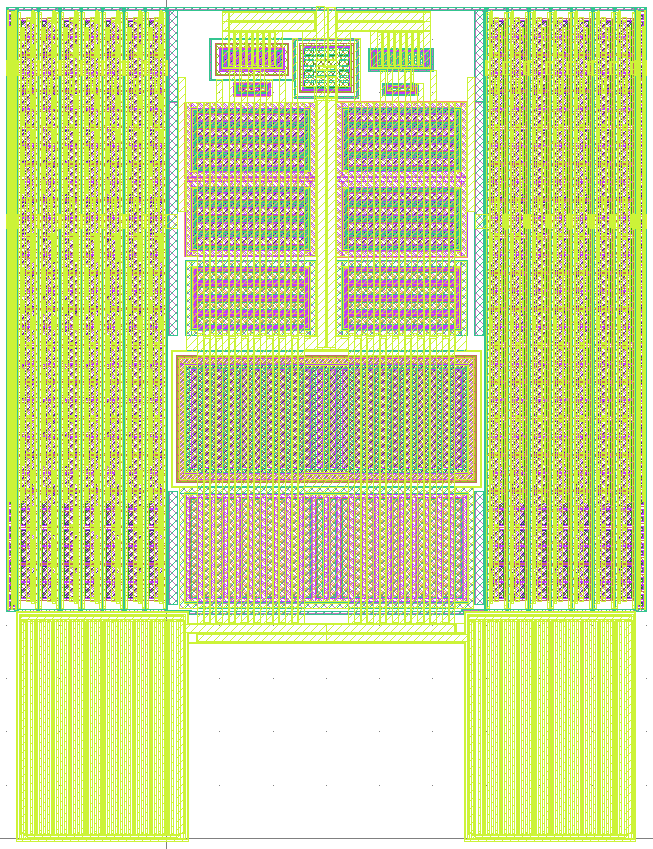
\includegraphics[height=\linewidth, angle=270]{figures/custom_guardsense_layout.png}
    \caption{A graphic representation of the layout of the custom guardsense pad}
    \label{fig:custom_guardsense_pad_layout}
\end{figure}


\subsection{Custom no ESD guarded pad}\label{no_esd_pad}

This is simply a bond pad with a guarded metal output.
No device whatsoever are connected to the input, which means that it has no ESD protection, but also minimal leakage on its own.
This pad is used anytime there is a device characterization pin, so that the measurement correspond to the actual device, and not the ESD protection circuitry.
In order to comply with antenna rules, it has sometime been necessary to route the signal up and down to upper metal layers  to comply with antenna rules.
An unconnected custom no ESD guarded pad is implemented in \ref{pad_leak_empty}, such that it will be possible to have a reference to other measurements.

\begin{figure}
    \centering
    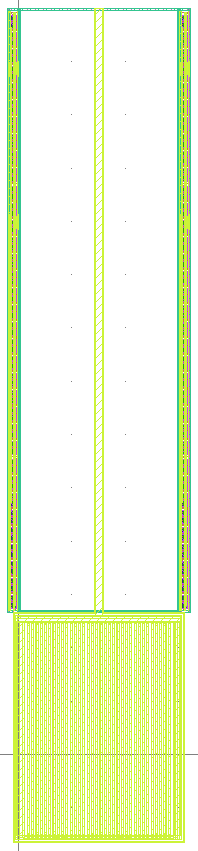
\includegraphics[height=\linewidth, angle=270]{figures/custom_no_esd_pad_layout.png}
    \caption{A graphic representation of the layout of the custom no esd pad}
    \label{fig:custom_no_esd_pad_layout}
\end{figure}


\section{Device Descriptions (by Device)}

% -------------------------------------------------------------------------
\subsection{MIMCAP\_MAX\_PERIM}\label{mimcap_max_perim}
\subsubsection{Description}
MIM capacitor of ($256\times16$\SI{}{\micro\meter} and \SI{8192}{\femto\farad}).
Its high perimeter geometry is to study the effect of perimeter in the MIM capacitor leakage.
It will be compared against \ref{mimcap_min_perim}.

\subsubsection{Pins (array)}
\[
\begin{array}{lll}
\#99, & \texttt{Guard}\\
\#100& \texttt{Pin 2}\\
\#1  & \texttt{Pin 1}\\
\end{array}
\]
Pin 1 connects to the lower plate, pin 2 to the upper plate.

\subsubsection{Diagram}
\begin{figure}[htp]
\centering
\begin{circuitikz}
  \draw
    (0,0) node[ocirc,label=left:{Pin 1}] (t1) {}
    (0,-3) node[ocirc,label=left:{Pin 2}] (t2) {}
    (0,-1.5) node[ocirc,label=left:{Guard}] (g) {}
    (t1) to[short] (2,0)
    (t2) to[short] (2,-3)
    (2,0) to[C,l=$C_{\mathrm{MIM}}\approx\SI{8192}{\femto\farad}$] (2,-3)
  ;
\end{circuitikz}
\caption{MIM capacitor (MAX\_PERIM) with guard.}
\end{figure}

% -------------------------------------------------------------------------
\subsection{MIMCAP\_MIN\_PERIM}\label{mimcap_min_perim}
\subsubsection{Description}
MIM capacitor of ($64\times64$\SI{}{\micro\meter} and \SI{8192}{\femto\farad}).
Its minimal perimeter geometry is to study the effect of perimeter in the MIM capacitor leakage.
It will be compared against \ref{mimcap_max_perim}.

\subsubsection{Pins (array)}
\[
\begin{array}{lll}
\#2 & \texttt{Pin 2}\\
\#3 & \texttt{Pin 1}\\
\#4 & \texttt{Guard}\\
\end{array}
\]
Pin 1 connects to the lower plate, pin 2 to the upper plate.

\subsubsection{Diagram}
\begin{figure}[htp]
\centering
\begin{circuitikz}
  \draw
    (0,0) node[ocirc,label=left:{Pin 1}] (t1) {}
    (0,-3) node[ocirc,label=left:{Pin 2}] (t2) {}
    (0,-1.5) node[ocirc,label=left:{Guard}] (g) {}
    (t1) to[short] (2,0)
    (t2) to[short] (2,-3)
    (2,0) to[C,l=$C_{\mathrm{MIM}}\approx\SI{8192}{\femto\farad}$] (2,-3)
  ;
\end{circuitikz}
\caption{MIM capacitor (MIN\_PERIM) with guard.}
\end{figure}

\subsection{GUARD\_LEAKAGE}\label{guard_leakage}
\subsubsection{Description}
This is a guarded line of $1041\times 3$ \SI{}{\micro\meter} in metal XXX.
It is guarded independently on the top, bottom and sides.
These guard planes can be swept in relation to the hot so that the influence of guarding in silicon can be measured.

\subsubsection{Pins (array)}
\[
\begin{array}{lll}
    \#14 & \texttt{Top guard plane}\\
    \#15 & \texttt{Bottom guard plane}\\
    \#16 & \texttt{Side guard traces}\\
    \#17 & \texttt{Hot}\\
    \#18 & \texttt{Guard of the hot bondpad}\\
\end{array}
\]

\subsubsection{Diagram}
\begin{circuitikz}
  \draw
    (0,4) node[ocirc,label=left:{Top guard}] (top) {}
    (0,3) node[ocirc,label=left:{Side guard}] (side) {}
    (0,2) node[ocirc,label=left:{Hot}] (hot) {}
    (0,0) node[ocirc,label=left:{Bottom guard}] (bottom) {}
    (hot) -- (8,2)
    (side) -- (9,3) -- (9,1) -- (0,1)
    (bottom) -- (8,0)
    (top) -- (8, 4)
  ;
\end{circuitikz}

\subsection{PAD\_ESD\_GUARDSENSE}\label{pad_esd_guardsense}
\subsubsection{Description}

Evaluate guard+sense approach and the ability to trim guard voltage using sense leakage.
See \ref{guardsense_pad} for details on the internal of the guardsense pad.
The purpose of the inverters is to measure up to what sort of ESD pulse the gate of the internal low voltage transistors making up the inverters can survive.

\subsubsection{Pins (array)}
\[
\begin{array}{lll}
    \#21 & \texttt{Inverted hot output}\\
    \#22 & \texttt{Inverted sense output}\\
    \#23 & \texttt{Sense input}\\
    \#25 & \texttt{Hot input}\\
    \#30 & \texttt{Guard}\\
\end{array}
\]

\subsubsection{Diagram}
\begin{circuitikz}
% Rails (moved up/down to avoid collisions)
\draw (0,7) node[vcc]{VDD} -- (13,7);
\draw (0,-1) node[ground]{VSS} -- (13,-1);

% ---------------- GuardSense PAD (black box) ----------------
% Black box
\draw (2,1) rectangle (7,5);
\node[align=center] at (4.5,3) {\textbf{GuardSense}\\\textbf{ESD Pad}};

% Left-side ports
\draw (1,4.2) node[ocirc,label=left:{PAD}]   (PAD)   {} -- (2,4.2);
\draw (1,1.8) node[ocirc,label=left:{SENSE}] (SENSE) {} -- (2,1.8);

% Right-side ports (unnamed, as requested)
\draw (7,4.2) node[ocirc] (PAD_INT)   {};
\draw (7,1.8) node[ocirc] (SENSE_INT) {};

% Optional GUARD port
\draw (1,3) node[ocirc,label=left:{GUARD}] (GUARD) {} -- (2,3);

% ---------------- Inverters ----------------
\draw (PAD_INT) ++(1.2,0) node[not port, anchor=in] (inv_pad) {};
\draw (SENSE_INT) ++(1.2,0) node[not port, anchor=in] (inv_sense) {};

\draw (PAD_INT) -- (inv_pad.in);
\draw (SENSE_INT) -- (inv_sense.in);

% ---------------- Separate outputs ----------------
\draw (inv_pad.out)   -- ++(1.4,0) node[ocirc,label=right:{$\overline{\mathrm{PAD}}$}]   (PADB)   {};
\draw (inv_sense.out) -- ++(1.4,0) node[ocirc,label=right:{$\overline{\mathrm{SENSE}}$}] (SENSEB) {};

\end{circuitikz}

\subsection{PAD\_ESD\_GUARD}\label{pad_esd_guard}
\subsubsection{Description}
Baseline custom guarded ESD pad without sense line.
The purpose of the inverter is to evaluate the robustness of the internal low-voltage inverter gate under ESD stress at the pad input.

\subsubsection{Pins (array)}
\[
\begin{array}{lll}
    \#27 & \texttt{Inverted hot output}\\
    \#29 & \texttt{Hot input}\\
    \#30 & \texttt{Guard}\\
\end{array}
\]

\subsubsection{Diagram}

\begin{circuitikz}
% Rails (kept clear of the symbols)
\draw (0,7) node[vcc]{VDD} -- (13,7);
\draw (0,-1) node[ground]{VSS} -- (13,-1);

% ---------------- Guarded ESD PAD (black box) ----------------
\draw (2,1) rectangle (7,5);
\node[align=center] at (4.5,3) {\textbf{Guarded}\\\textbf{ESD Pad}};

% Left-side port
\draw (1,4) node[ocirc,label=left:{PAD}] (PAD) {} -- (2,4);

% Right-side internal node (unnamed)
\draw (7,3) node[ocirc] (PAD_INT) {};

% Guard port
\draw (1,2) node[ocirc,label=left:{GUARD}] (GUARD) {} -- (2,2);

% ---------------- Inverter on output ----------------
\draw (PAD_INT) ++(1.2,0) node[not port, anchor=in] (inv_pad) {};
\draw (PAD_INT) -- (inv_pad.in);

% Output
\draw (inv_pad.out) -- ++(1.4,0) node[ocirc,label=right:{$\overline{\mathrm{PAD}}$}] (PADB) {};
\end{circuitikz}

\subsection{ESD\_DIODE\_VDD}\label{esd_diode_vdd}
\subsubsection{Purpose}
Standalone foundry-provided vdd esd diode for ultralow current I-V characterization.

\subsubsection{Pins (array)}

\[
\begin{array}{lll}
    \#49 & \texttt{Cathode}\\
    \#51 & \texttt{Anode}\\
    \#52 & \texttt{Guard}\\
\end{array}
\]

\subsubsection{Diagram}

\begin{circuitikz}
  \draw
    (0,3) node[ocirc,label=left:{Anode}] (a) {}
    (0,0) node[ocirc,label=left:{Cathode}] (k) {}
    (0,1.5) node[ocirc,label=left:{Guard}] (g) {}
    (a) -- (1,3) to[D,l=VDD ESD diode]  (1,0) -- (k)
  ;
\end{circuitikz}

% -------------------------------------------------------------------------
\subsection{ESD\_DIODE\_VSS}\label{esd_diode_vss}
\subsubsection{Purpose}
Standalone foundry-provided VSS ESD diode for ultralow current I-V characterization.
The anode is shorted to VSS through the substrate.

\subsubsection{Pins (array)}

\[
\begin{array}{lll}
    \#50 & \texttt{Cathode}\\
    \#52 & \texttt{Guard}\\
\end{array}
\]

\subsubsection{Diagram}

\begin{circuitikz}
  \draw
    % VSS as a named net (no port circle)
    (1,3) node[right]{VSS} (a) {}

    (0,0) node[ocirc,label=left:{Cathode}] (k) {}
    (0,1.5) node[ocirc,label=left:{Guard}] (g) {}

    (1,3) to[D,l=VSS ESD diode] (1,0) -- (k)
  ;
\end{circuitikz}


% -------------------------------------------------------------------------
\subsection{Guarded HV/LV NFET/PFET, W=0.75um L=0.7um} \label{transistors}
\subsubsection{Description}

Direct access to D/G/S for transistor leakage characterization under guarding.
No ESD pads were used on signal of interest, but an up and down metal break is made to comply with antenna rules.

\subsubsection{Pins (array)}
\[
\begin{array}{llll}
\text{Device type} & \text{Drain} & \text{Gate} & \text{Source} \\
\hline
\text{HV PFET:} & \#56 & \#57 & \#58 \\
\text{HV NFET:} & \#59 & \#60 & \#61 \\
\text{LV PFET:} & \#62 & \#63 & \#64 \\
\text{LV NFET:} & \#65 & \#66 & \#67 \\
\end{array}
\]
Pin \#55 and \#68 (internally shorted) as used as guard for all transistor structures.

\subsubsection{Diagram (generic, horizontal MOS symbol)}

\begin{circuitikz}
  \draw
    (0,0) node[ocirc,label=left:{Drain}] (d) {}
    (0,-1) node[ocirc,label=left:{Gate}] (g) {}
    (0,-2) node[ocirc,label=left:{Source}] (s) {}
    (0,1) node[ocirc,label=left:{Guard (\#55)}] (guard) {}
    (0,-3) node[ocirc,label=left:{Guard (\#68)}] (guard2) {}

    (guard) -- (5,1) |- (guard2)

    % Use a horizontal nmos; keep connections vertical/horizontal only
    (3,-1) node[nmos] (M) {}

    (d) -| (M.D)
    (g) -- (M.G)
    (s) -| (M.S)
  ;
\end{circuitikz}

\subsection{PAD\_LEAK\_EMPTY}\label{pad_leak_empty}
\subsubsection{Description}
Custom no ESD bondpad, presented in \ref{no_esd_pad} connected to nothing.
It will be used as a reference to all other measurement involving this pad.

\subsubsection{Pins (array)}
\[
\begin{array}{lll}
    \#71 & \texttt{Guard}\\
    \#72 & \texttt{Hot}\\
    \#80 & \texttt{Guard}\\
\end{array}
\]
Guards are internally shorted together.

\subsubsection{Diagram}

\begin{circuitikz}
  % Bondpad blackbox
  \draw (1,-1) rectangle (5,1);
  \node[align=center] at (3,0) {\textbf{Bondpad}};

  % Ports on the left: guard (top), hot (middle), guard (bottom)
  \draw (0, 1.5) node[ocirc,label=left:{GUARD}] (gT) {};
  \draw (0, 0.0) node[ocirc,label=left:{HOT}]       (hot) {};
  \draw (0,-1.5) node[ocirc,label=left:{GUARD}] (gB) {};

  % Connect HOT to bondpad
  \draw (hot) -- (1,0);

  % (Optional) show guard lines approaching the bondpad region
  \draw (5,0) -- (7.5,0);
  \draw (gT) -- (8,1.5) |- (gB);
\end{circuitikz}

% -------------------------------------------------------------------------
\subsection{PAD\_LEAK\_GUARDSENSE}
\subsubsection{Purpose}

Implements the custom guardsense pad with nothing connected to its output.
This allows for measuring the intrinsic leakage of the device.
It could also be used for ESD testing, to characterize the robustness of the pad structure itself, as opposed to \ref{pad_esd_guardsense}, which characterizes its ability to protect the core transistors.

\subsubsection{Pins (array)}
\[
\begin{array}{lll}
    \#71 & \texttt{Guard}\\
    \#73 & \texttt{Sense input}\\
    \#75 & \texttt{Hot input}\\
    \#80 & \texttt{Guard}\\
\end{array}
\]
Guards are internally shorted together.

\subsubsection{Diagram}
\begin{circuitikz}
% Rails (moved up/down to avoid collisions)
\draw (0,7) node[vcc]{VDD} -- (13,7);
\draw (0,-1) node[ground]{VSS} -- (13,-1);

% ---------------- GuardSense PAD (black box) ----------------
% Black box
\draw (2,1) rectangle (7,5);
\node[align=center] at (4.5,3) {\textbf{GuardSense}\\\textbf{ESD Pad}};

% Left-side ports
\draw (1,4.2) node[ocirc,label=left:{PAD}]   (PAD)   {} -- (2,4.2);
\draw (1,1.8) node[ocirc,label=left:{SENSE}] (SENSE) {} -- (2,1.8);

% Right-side ports (unnamed, as requested)
\draw (7,4.2) node[ocirc] (PAD_INT)   {};
\draw (7,1.8) node[ocirc] (SENSE_INT) {};

% Optional GUARD port
\draw (1,3) node[ocirc,label=left:{GUARD}] (GUARD) {} -- (2,3);


\end{circuitikz}

% -------------------------------------------------------------------------
\subsection{PAD\_LEAK\_GUARD}
\subsubsection{Purpose}
Implements the custom guard pad with nothing connected to its output.
This allows for measuring the intrinsic leakage of the device.
It could also be used for ESD testing, to characterize the robustness of the pad structure itself, as opposed to \ref{pad_esd_guard}, which characterizes its ability to protect the core transistors.

\subsubsection{Pins (array)}
\[
\begin{array}{lll}
    \#71 & \texttt{Guard}\\
    \#77 & \texttt{Hot input}\\
    \#80 & \texttt{Guard}\\
\end{array}
\]
Guards are internally shorted together.

\subsubsection{Diagram}

\begin{circuitikz}
% Rails (kept clear of the symbols)
\draw (0,7) node[vcc]{VDD} -- (13,7);
\draw (0,-1) node[ground]{VSS} -- (13,-1);

% ---------------- Guarded ESD PAD (black box) ----------------
\draw (2,1) rectangle (7,5);
\node[align=center] at (4.5,3) {\textbf{Guarded}\\\textbf{ESD Pad}};

% Left-side port
\draw (1,4) node[ocirc,label=left:{PAD}] (PAD) {} -- (2,4);

% Right-side internal node (unnamed)
\draw (7,3) node[ocirc] (PAD_INT) {};

% Guard port
\draw (1,2) node[ocirc,label=left:{GUARD}] (GUARD) {} -- (2,2);

\end{circuitikz}

\subsection{PAD\_LEAK\_ASIG}

\subsubsection{Description}

Implements the foundry provided analog pad with nothing connected to its output.
The bondpad itself is guarded, but the internal structures are not, as they are left untouched.
This allows for measuring the intrinsic leakage of the pad.
It could also be used for ESD testing, to characterize the robustness of the pad structure itself.

\subsubsection{Pins (array)}
\[
\begin{array}{lll}
    \#71 & \texttt{Guard}\\
    \#77 & \texttt{Hot input}\\
    \#80 & \texttt{Guard}\\
\end{array}
\]
Guards are internally shorted together.

\subsubsection{Diagram (abstract, horizontal)}
\begin{circuitikz}
% Rails (kept clear of the symbols)
\draw (0,7) node[vcc]{VDD} -- (13,7);
\draw (0,-1) node[ground]{VSS} -- (13,-1);

% ---------------- Guarded ESD PAD (black box) ----------------
\draw (2,1) rectangle (7,5);
\node[align=center] at (4.5,3) {\textbf{Foundry-provided}\\\textbf{Analog ESD Pad}};

% Left-side port
\draw (1,3) node[ocirc,label=left:{PAD}] (PAD) {} -- (2,3);

% Right-side internal node (unnamed)
\draw (7,3) node[ocirc] (PAD_INT) {};

% Guard port
\draw (1,5) node[ocirc,label=left:{GUARD}] (GUARD) {};

\end{circuitikz}

\subsection{CHARGE\_PUMP}\label{charge_pump}
\subsubsection{Purpose}
Implements the fifty nifty pico ampere current source.

H. Pretl and M. Eberlein, IEEE SSC Magazine 2021 (DOI: 10.1109/MSSC.2021.3088968);

Its operation is described in detail in

U. Cilingiroglu et al., IEEE JSSC 2003 (DOI: 10.1109/JSSC.2002.806282).

Two matched PMOS transistors with separate gates enabling opposite polarity operation to reduce injected noise. Implemented with PMOS W=\SI{40}{\micro\meter}, L=\SI{1}{\micro\meter} (provided).

\subsubsection{Pins (array)}
\[
\begin{array}{lll}
    \#83 & \texttt{Guard}\\
    \#84 & \texttt{Gate of transistor 2}\\
    \#85 & \texttt{VS (drain and source of both transistors)}\\
    \#86 & \texttt{Gate of transistor 1}\\
    \#87 & \texttt{VW (bulk of both transistors)}\\
\end{array}
\]

\subsubsection{Diagram}

\begin{circuitikz}
  \draw
    % Left ports (align gate ports to the actual gate y-positions)
    (0, 0)   node[ocirc,label=left:{VS}] (vs) {}
    (0, 1.1) node[ocirc,label=left:{G1}] (g1) {}
    (0,-1.1) node[ocirc,label=left:{G2}] (g2) {}

    % Right ports
    (6, 0)   node[ocirc,label=right:{VW (bulk/well)}] (vw) {}
    (0,-2.6) node[ocirc,label=left:{Guard}] (guard) {}

    % Two PMOS (stacked vertically)
    (4, 1.1) node[pmos] (P1) {}
    (4,-1.1) node[pmos] (P2) {}
  ;

  % VS bus
  \draw (vs) -- (2,0) coordinate (vsbus);

  % Tie D and S of each PMOS to VS
  \draw (vsbus) |- (P1.D);
  \draw (vsbus) |- (P2.D);

  % For the "middle" connections (the ones that run down/up to the VS bus),
  % add explicit junction dots where they meet the horizontal VS bus.
  \draw (2,0.33)  node[circ] {} |- (P1.S);
  \draw (2,-0.33)  node[circ] {} |- (P2.S);

  % Gates
  \draw (g1) -- (P1.G);
  \draw (g2) -- (P2.G);

  % Bulk/well
  \draw (P1.B) -| (vw);
  \draw (P2.B) -| (vw);

  % (optional) conceptual leakage from VS to guard
  % \draw (vs) to[R,l=$R_{\mathrm{leak}}$,dashed] (guard);
\end{circuitikz}

\section{Bonding Diagram}
\subsection{Die / Pad Dimensions}

The ASIC measures \SI{1936}{\micro\meter} by \SI{5122}{\micro\meter}.
Its height is \SI{250}{\micro\meter}.

The bondpads measure \SI{78}{\micro\meter} by \SI{100}{\micro\meter}. Their pitch is \SI{105}{\micro\meter}. The outward edge of the pad is \SI{26}{\micro\meter} away from the sealring.


\subsection{Bonding Diagram and Recommended PCB Footprint}

As the ASIC is composed of many pads, and the ultra-low current nature of the teststructures require a certain spacing between the PCB pads, two bonding diagrams have been made, each one allowing access to a subset of the test structures.

\begin{figure}[t]
\centering
\begin{subfigure}{.5\textwidth}
  \centering
  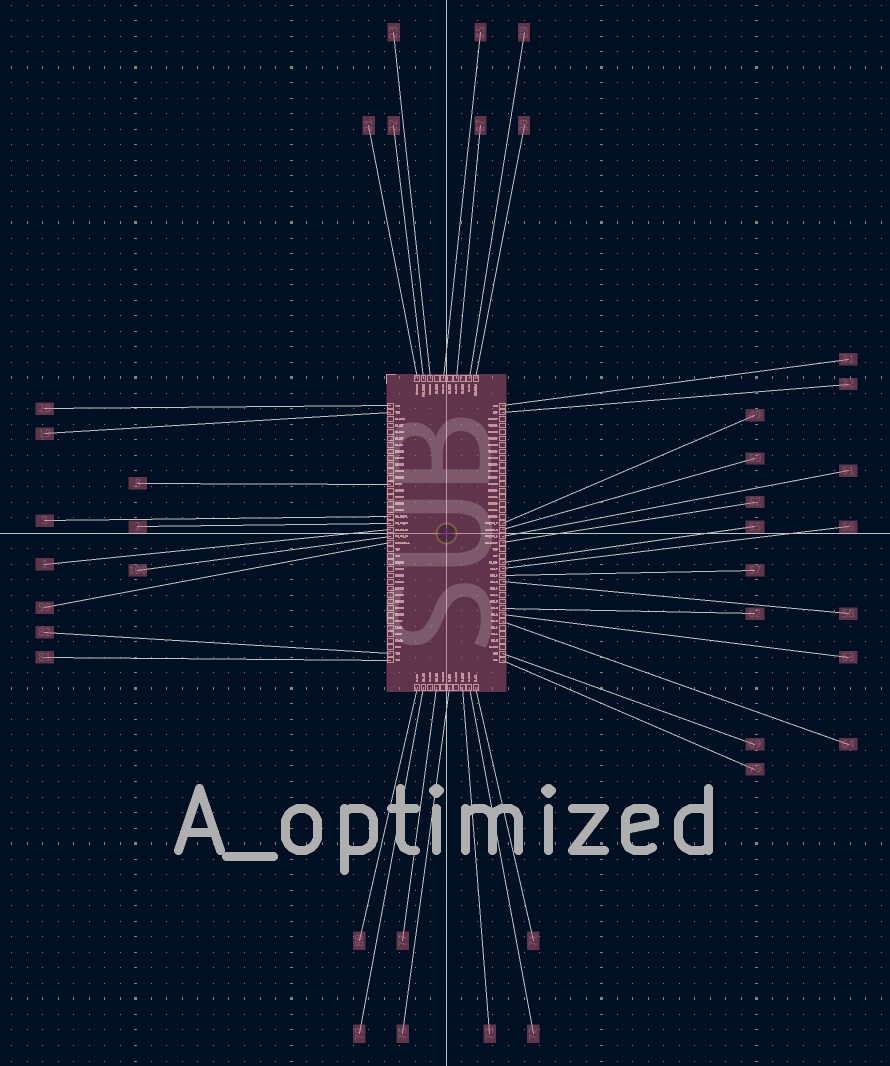
\includegraphics[width=.8\linewidth]{figures/bonding_A.png}
  \caption{Bonding diagram variant A}
  \label{fig:sub1}
\end{subfigure}%
\begin{subfigure}{.5\textwidth}
  \centering
  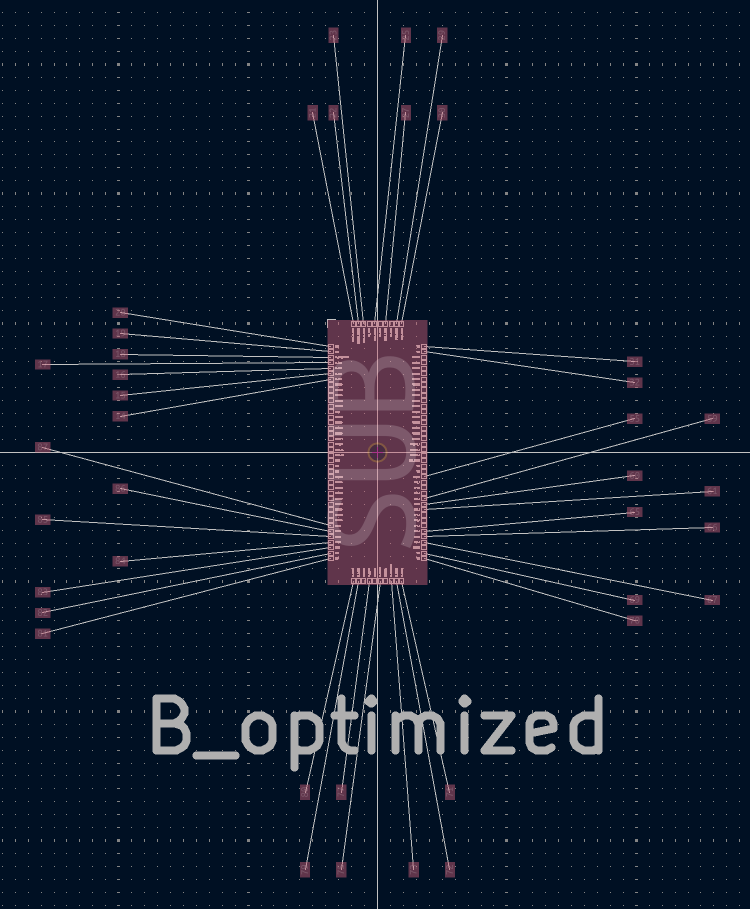
\includegraphics[width=.8\linewidth]{figures/bonding_B.png}
  \caption{Bonding diagram variant B}
  \label{fig:sub2}
\end{subfigure}
\caption{trident-gf180-teststructures bonding diagrams}
\label{fig:test}
\end{figure}

\begin{figure}
\begin{longtable}{l r l l l l l l}
\toprule
\#  & side & bondpad\_x & bondpad\_y  & pcbpad\_x & pcbpad\_y & length\_mm  & angle  [°] \\

\midrule
1 & WEST & -0.903 & 0.0525 & -6.468 & -0.5 & 5.592359 & -5.67 \\
2 & WEST & -0.903 & 0.1575 & -4.968 & 0.1 & 4.065407 & -0.81 \\
3 & WEST & -0.903 & 0.2625 & -6.468 & 0.2 & 5.565351 & -0.64 \\
8 & WEST & -0.903 & 0.7875 & -4.968 & 0.8 & 4.065019 & 0.18 \\
19 & WEST & -0.903 & 1.9425 & -6.468 & 1.6 & 5.57553 & -3.52 \\
20 & WEST & -0.903 & 2.0475 & -6.468 & 2 & 5.565203 & -0.49 \\
21 & NORTH & -0.4725 & 2.485 & -1.25 & 6.561 & 4.149492 & -10.8 \\
22 & NORTH & -0.3675 & 2.485 & -0.85 & 6.561 & 4.104459 & -6.75 \\
23 & NORTH & -0.2625 & 2.485 & -0.85 & 8.061 & 5.606865 & -6.01 \\
25 & NORTH & -0.0525 & 2.485 & 0.55 & 8.061 & 5.608456 & 6.17 \\
27 & NORTH & 0.1575 & 2.485 & 0.55 & 6.561 & 4.094854 & 5.5 \\
29 & NORTH & 0.3675 & 2.485 & 1.25 & 8.061 & 5.645404 & 8.99 \\
30 & NORTH & 0.4725 & 2.485 & 1.25 & 6.561 & 4.149492 & 10.8 \\
31 & EAST & 0.903 & 2.0475 & 6.468 & 2.8 & 5.615646 & -7.7 \\
32 & EAST & 0.903 & 1.9425 & 6.468 & 2.4 & 5.583774 & -4.7 \\
49 & EAST & 0.903 & 0.1575 & 4.968 & 1.9 & 4.422729 & -23.2 \\
50 & EAST & 0.903 & 0.0525 & 4.968 & 1.2 & 4.223859 & -15.76 \\
51 & EAST & 0.903 & -0.0525 & 6.468 & 1 & 5.663654 & -10.71 \\
52 & EAST & 0.903 & -0.1575 & 4.968 & 0.5 & 4.117831 & -9.19 \\
55 & EAST & 0.903 & -0.4725 & 4.968 & 0.1 & 4.105116 & -8.02 \\
56 & EAST & 0.903 & -0.5775 & 6.468 & 0.1 & 5.606089 & -6.94 \\
57 & EAST & 0.903 & -0.6825 & 4.968 & -0.6 & 4.065837 & -1.16 \\
58 & EAST & 0.903 & -0.7875 & 6.468 & -1.3 & 5.588549 & 5.26 \\
62 & EAST & 0.903 & -1.2075 & 4.968 & -1.3 & 4.066052 & 1.3 \\
63 & EAST & 0.903 & -1.3125 & 6.468 & -2 & 5.607306 & 7.04 \\
64 & EAST & 0.903 & -1.4175 & 6.468 & -3.4 & 5.907583 & 19.61 \\
69 & EAST & 0.903 & -1.9425 & 4.968 & -3.4 & 4.318395 & 19.73 \\
70 & EAST & 0.903 & -2.0475 & 4.968 & -3.8 & 4.426678 & 23.32 \\
71 & SOUTH & 0.4725 & -2.485 & 1.4 & -6.561 & 4.180195 & -12.82 \\
72 & SOUTH & 0.3675 & -2.485 & 1.4 & -8.061 & 5.670788 & -10.49 \\
73 & SOUTH & 0.2625 & -2.485 & 0.7 & -8.061 & 5.593137 & -4.49 \\
75 & SOUTH & 0.0525 & -2.485 & -0.7 & -8.061 & 5.626547 & 7.69 \\
77 & SOUTH & -0.1575 & -2.485 & -0.7 & -6.561 & 4.111944 & 7.58 \\
79 & SOUTH & -0.3675 & -2.485 & -1.4 & -8.061 & 5.670788 & 10.49 \\
80 & SOUTH & -0.4725 & -2.485 & -1.4 & -6.561 & 4.180195 & 12.82 \\
81 & WEST & -0.903 & -2.0475 & -6.468 & -2 & 5.565203 & 0.49 \\
82 & WEST & -0.903 & -1.9425 & -6.468 & -1.6 & 5.57553 & 3.52 \\
99 & WEST & -0.903 & -0.1575 & -6.468 & -1.2 & 5.661805 & -10.61 \\
100 & WEST & -0.903 & -0.0525 & -4.968 & -0.6 & 4.101705 & -7.67 \\

\bottomrule
\end{longtable}
\caption{Bonding wire information for variant A}

\end{figure}

\begin{figure}
\begin{longtable}{l r l l l l l l}
\toprule
\#  & side & bondpad\_x & bondpad\_y  & pcbpad\_x & pcbpad\_y & length\_mm  & angle  [°] \\

\midrule
14 & WEST & -0.903 & 1.4175 & -4.968 & 0.7 & 4.127836 & -10.01 \\
15 & WEST & -0.903 & 1.5225 & -4.968 & 1.1 & 4.086898 & -5.93 \\
16 & WEST & -0.903 & 1.6275 & -4.968 & 1.5 & 4.066999 & -1.8 \\
17 & WEST & -0.903 & 1.7325 & -6.468 & 1.7 & 5.565095 & -0.33 \\
18 & WEST & -0.903 & 1.8375 & -4.968 & 1.9 & 4.06548 & 0.88 \\
19 & WEST & -0.903 & 1.9425 & -4.968 & 2.3 & 4.08069 & 5.03 \\
20 & WEST & -0.903 & 2.0475 & -4.968 & 2.7 & 4.117035 & 9.12 \\
21 & NORTH & -0.4725 & 2.485 & -1.25 & 6.561 & 4.149492 & -10.8 \\
22 & NORTH & -0.3675 & 2.485 & -0.85 & 6.561 & 4.104459 & -6.75 \\
23 & NORTH & -0.2625 & 2.485 & -0.85 & 8.061 & 5.606865 & -6.01 \\
25 & NORTH & -0.0525 & 2.485 & 0.55 & 8.061 & 5.608456 & 6.17 \\
27 & NORTH & 0.1575 & 2.485 & 0.55 & 6.561 & 4.094854 & 5.5 \\
29 & NORTH & 0.3675 & 2.485 & 1.25 & 8.061 & 5.645404 & 8.99 \\
30 & NORTH & 0.4725 & 2.485 & 1.25 & 6.561 & 4.149492 & 10.8 \\
31 & EAST & 0.903 & 2.0475 & 4.968 & 1.75 & 4.075872 & 4.19 \\
32 & EAST & 0.903 & 1.9425 & 4.968 & 1.35 & 4.107953 & 8.29 \\
55 & EAST & 0.903 & -0.4725 & 4.968 & 0.65 & 4.217135 & -15.44 \\
59 & EAST & 0.903 & -0.8925 & 6.468 & 0.65 & 5.774819 & -15.49 \\
60 & EAST & 0.903 & -0.9975 & 4.968 & -0.45 & 4.101705 & -7.67 \\
61 & EAST & 0.903 & -1.1025 & 6.468 & -0.75 & 5.576153 & -3.62 \\
65 & EAST & 0.903 & -1.5225 & 4.968 & -1.15 & 4.082032 & -5.24 \\
66 & EAST & 0.903 & -1.6275 & 6.468 & -1.45 & 5.56783 & -1.83 \\
67 & EAST & 0.903 & -1.7325 & 6.468 & -2.85 & 5.676093 & 11.35 \\
69 & EAST & 0.903 & -1.9425 & 4.968 & -2.85 & 4.165067 & 12.58 \\
70 & EAST & 0.903 & -2.0475 & 4.968 & -3.25 & 4.239131 & 16.48 \\
71 & SOUTH & 0.4725 & -2.485 & 1.4 & -6.561 & 4.180195 & -12.82 \\
72 & SOUTH & 0.3675 & -2.485 & 1.4 & -8.061 & 5.670788 & -10.49 \\
73 & SOUTH & 0.2625 & -2.485 & 0.7 & -8.061 & 5.593137 & -4.49 \\
75 & SOUTH & 0.0525 & -2.485 & -0.7 & -8.061 & 5.626547 & 7.69 \\
77 & SOUTH & -0.1575 & -2.485 & -0.7 & -6.561 & 4.111944 & 7.58 \\
79 & SOUTH & -0.3675 & -2.485 & -1.4 & -8.061 & 5.670788 & 10.49 \\
80 & SOUTH & -0.4725 & -2.485 & -1.4 & -6.561 & 4.180195 & 12.82 \\
81 & WEST & -0.903 & -2.0475 & -6.468 & -3.5 & 5.751433 & -14.63 \\
82 & WEST & -0.903 & -1.9425 & -6.468 & -3.1 & 5.684103 & -11.75 \\
83 & WEST & -0.903 & -1.8375 & -6.468 & -2.7 & 5.631441 & -8.81 \\
84 & WEST & -0.903 & -1.7325 & -4.968 & -2.1 & 4.081578 & -5.17 \\
85 & WEST & -0.903 & -1.6275 & -6.468 & -1.3 & 5.574628 & 3.37 \\
86 & WEST & -0.903 & -1.5225 & -4.968 & -0.7 & 4.147376 & 11.44 \\
87 & WEST & -0.903 & -1.4175 & -6.468 & 0.1 & 5.768191 & 15.25 \\


\bottomrule
\end{longtable}
\caption{Bonding wire information for variant B}

\end{figure}

\end{document}
